\documentclass[12pt]{article}

% This is the preamble, load any packages you're going to use here
\usepackage{physics} % provides lots of nice features and commands often used in physics, it also loads some other packages (like AMSmath)
\usepackage{siunitx} % typesets numbers with units very nicely
\usepackage{enumerate} % allows us to customize our lists
\usepackage{graphicx}



\begin{document}
\pagenumbering{gobble}% Remove page numbers (and reset to 1)

\title{EE 511 Computer Vision Assignment 1}
\author{B12015 Rohit Patiyal}
\date{\today}

\maketitle
\section*{Theory \& Steps}
	\subsection*{Vanishing Point}
 Vanishing point is the point in which receding parallel lines in perspective appear to converge.

	In order to find Vanishing point in a given image the following steps are to done :
    \begin{enumerate}
		\item{Gray Scaling the image to proceed for edge detection}
        \item{Edges are highlighted by converting to Black and white}
        \item{Hough transform is used to detect lines}
        \item{The point of intersection may be a vanishing point if the lines are actually parallel in 3D world coordinates}
        \item{Here we consider all points of intersection of lines having some threshold level of angle between them}
        \item{Only some intersection points which are vanishing points are inside the image, otherwise they are out of the image}
	\end{enumerate}
    
    \pagebreak
    
    \subsection*{Disparity}
		Disparity refers to the distance between two corresponding points in the left and right image of a stereo pair. 
        Steps for finding disparity are:
        \begin{enumerate}
		\item{For each pixel in left image search in nearby space of the right image.}
        \item{Use some criteria like Sum of absolute diff or Sum of Squared Sums or Normalized cross correlation over a patch of a window to find the best match}
        \item{This needs to be done only along the row for the given images setup}
        \item{Observe these distance (in pixels) by plotting these values as an image}
	\end{enumerate}
    
      \pagebreak
      

    \begin{figure}
    \section*{Observations}
    \section{Vanishing Point}
    \subsection{Image 1}
	\hspace{-3cm}
    \includegraphics{grill/res.png}
    In the 6th subplot we can see that based on the prominent lines in the image,
    we get some intersection points, Most of them are outside of the image which is justified because we do not see parallel lines converging withing the boundary of the image. Although there is a point near the left border which appears to be a valid vanishing point. 
	\end{figure}
   
    \begin{figure}  
    \subsection{Image 2}
	 \hspace{-3cm}
    \includegraphics{rail/res.png}
      Again in the last subplot we see that there is a convergence of the parallel railway lines in a perspective view and hence we obtain a point in the middle of the image as the vanishing point
	\end{figure}
  
     \begin{figure}  
    \subsection{Image 3}
	     \hspace{-3cm}
    \includegraphics{house/res.png}
    Here there are already lines which help in obtaining perspective lines and finding the intersection point. Although no vanishing point is visible in the image, we do get a point of intersection which actually appears because hough transform considered their lines as separate lines and an intersection point comes up.
	\end{figure}

	\pagebreak

  
		
    \begin{figure}[!htb]
      \section{Disparity Map}
    \subsection{Real World pair 1}
    \centering
    \begin{minipage}{.5\textwidth}
        \centering
        \includegraphics[width=0.7\linewidth]{pair1/scene_l.png}
        \caption{Left Camera Image }
        \label{fig:1}
    \end{minipage}%
    \begin{minipage}{0.5\textwidth}
        \centering
        
        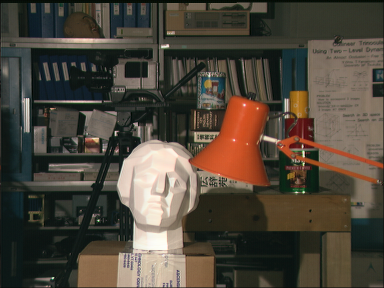
\includegraphics[width=0.7\linewidth]{pair1/scene_r.png}
        \caption{Right Camera Image}
        \label{fig:2}
    \end{minipage}
    
      \includegraphics[width=1\linewidth]{pair1/res.png}
      
      We can observe that we obtain very similar disparity maps for both 15 and 20 search space sizes. There is a significant difference between abs or sq diff and normalized cross correlation criteria images. Also it appears that the boundaries of object tend to have distorted disparity because they go inward of the plane near the boundaries.
\end{figure}
  
   
  \begin{figure}[!htb]
   \subsection{Generated pair 2}
    \centering
    \begin{minipage}{.5\textwidth}
        \centering
        \includegraphics[width=0.7\linewidth]{pair2/scene_l.png}
        \caption{Left Camera Image }
        \label{fig:3}
    \end{minipage}%
    \begin{minipage}{0.5\textwidth}
        \centering
        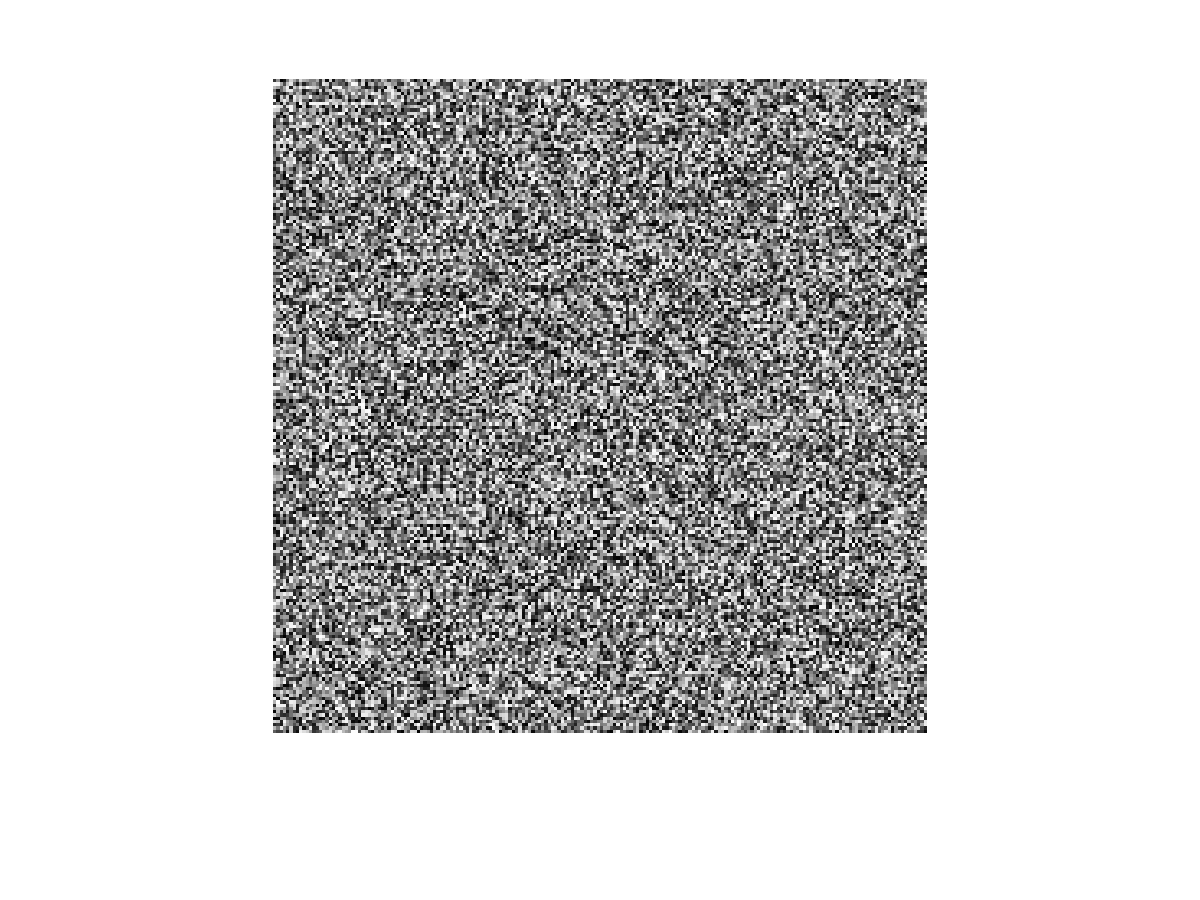
\includegraphics[width=0.7\linewidth]{pair2/scene_r.png}
        \caption{Right Camera Image}
        \label{fig:4}
    \end{minipage}
      
      \includegraphics[width=1\linewidth]{pair2/res.png}
      The generated pair of images does not show any significant difference between different matching criteria. Also it can be inferred that points close to camera tend to be brighter and hence brightness demonstrates the relative positions of the points along the depth.
\end{figure}

  

 
  \begin{figure}[!htb]
  \subsection{Real World pair 3}
    \centering
    \begin{minipage}{.5\textwidth}
        \centering
        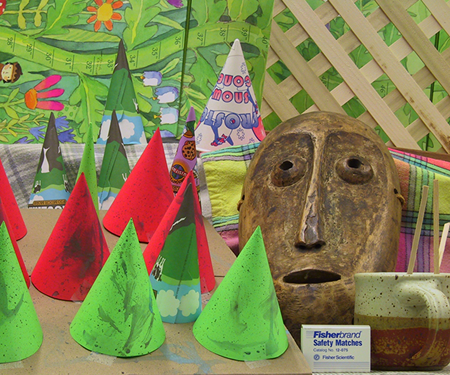
\includegraphics[width=0.7\linewidth]{pair3/im_l.png}
        \caption{Left Camera Image }
        \label{fig:5}
    \end{minipage}%
    \begin{minipage}{0.5\textwidth}
        \centering
        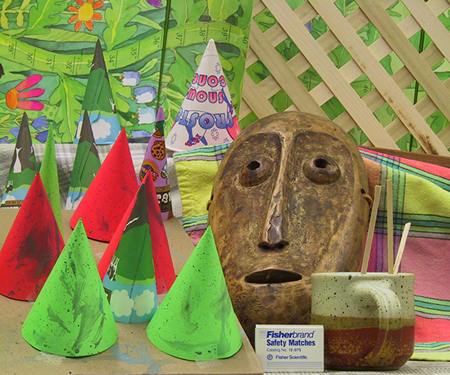
\includegraphics[width=0.7\linewidth]{pair3/im_r.png}
        \caption{Right Camera Image}
        \label{fig:6}
    \end{minipage}
      
      \includegraphics[width=1\linewidth]{pair3/res.png}
      This image produces very inaccurate results for the disparity irrespective of the criteria or the search-space size. This also paves the way for more complex algorithms for finding the disparity. For the standard row wise pattern matching, this image pair appears to be a hard case, yet, shapes of some objects are faintly visible.
    \end{figure}
 



\end{document}